\chapter{Training versus Testing}
\lecture{5}{23 Sep.}{}

\begin{prev}
    \autoref{thm:finite-hoeffding} closed the last chapter: if
    \(\mathcal{H} = \left\{ h_1, \dots , h_M \right\}\) is finite and \(N\) is
    large enough, then
    \[
        \mathbb{P}\left[ \abs{\Ein(g) - \Eout(g)} > \epsilon \right]
        \le 2 M \exp \left( -2 \epsilon^2 N \right)
    \]
    for whatever \(g\) the algorithm picks --- so if \(\mathcal{A}\) also finds
    a \(g\) with \(\Ein(g) \approx 0\), we get the PAC guarantee
    \(\Eout(g) \approx 0\) and learning is possible.
\end{prev}

The one hypothesis set we actually own is infinite. Perceptrons form a
continuum, \(M = \infty\), and the bound collapses to the statement that a
probability is at most \(\infty\). This chapter does not repair the proof; it
repairs the \emph{counting} inside it. \(M\) entered through a union bound over
\(M\) bad events, and a union bound is wasteful exactly when those events
overlap --- which, for a hypothesis set full of near-identical hypotheses, they
badly do. The honest count is not how many hypotheses \(\mathcal{H}\) contains
but how many \emph{kinds} of behaviour it can display on \(N\) fixed inputs.
That count is finite even when \(\mathcal{H}\) is not, and the chapter ends by
isolating the property that keeps it small.

\section{Recap and Preview}\label{sec:recap-preview}

\source{slides p.2--6}

\subsection{The `Statistical' Learning Flow}

The flow of \autoref{sec:real-learning} is worth putting down once more, now
with its conclusion written underneath it rather than argued towards.

\begin{center}
    \begin{adjustbox}{max width=\textwidth}
        \begin{tikzpicture}
            \node[mlbox, minimum width=4.4cm] (f) at (0,2.5)
                {unknown target function\\
                 \(f\colon \mathcal{X} \to \mathcal{Y}\)\\[2pt]
                 {\scriptsize (ideal credit approval formula)}};
            \node[mlbox, minimum width=2.6cm, draw=Dandelion!80!black,
                fill=Dandelion!12] (P) at (5.4,2.5)
                {unknown\\\(P\) on \(\mathcal{X}\)};
            \node[mlbox, minimum width=5.2cm] (D) at (0,0)
                {training examples\\
                 \(\mathcal{D}\colon (\bm{x}_1, y_1), \dots , (\bm{x}_N, y_N)\)\\[2pt]
                 {\scriptsize (historical records in bank)}};
            \node[mlop, minimum width=2.4cm] (A) at (5.4,0)
                {learning\\algorithm\\\(\mathcal{A}\)};
            \node[mlbox, minimum width=4.4cm] (g) at (10.2,0)
                {final hypothesis\\\(g \approx f\)\\[2pt]
                 {\scriptsize (`learned' formula to be used)}};
            \node[mlbox, minimum width=3.4cm] (H) at (5.4,-2.4)
                {hypothesis set\\\(\mathcal{H}\)\\[2pt]
                 {\scriptsize (set of candidate formulas)}};
            \draw[mlarrow] (f) -- (D);
            \draw[mlarrow, draw=Dandelion!80!black, dashed] (P) -- (D)
                node[pos=0.58, font=\scriptsize, fill=white, inner sep=1.5pt]
                {\(\bm{x}_1, \bm{x}_2, \dots , \bm{x}_N\)};
            \draw[mlarrow, draw=Dandelion!80!black, dashed] (P.east) -- (g.north)
                node[pos=0.55, font=\scriptsize, fill=white, inner sep=1.5pt]
                {\(\bm{x}\)};
            \draw[mlarrow] (D) -- (A);
            \draw[mlarrow] (A) -- (g);
            \draw[mlarrow] (H) -- (A);
            \node[draw=Dandelion!80!black, fill=Dandelion!10, rounded corners=3pt,
                inner sep=6pt] at (10.2,-2.4)
                {\(\Eout(g) \underbrace{\approx}_{\text{test}}
                  \Ein(g) \underbrace{\approx}_{\text{train}} 0\)};
        \end{tikzpicture}
    \end{adjustbox}
\end{center}

The two \(\approx\) signs are of completely different kinds, and the label under
each says which. The right-hand one is \emph{earned}: the algorithm works on
\(\mathcal{D}\) until the in-sample error is small, and nothing stops it from
trying. The left-hand one is \emph{granted}: no amount of work on
\(\mathcal{D}\) can establish it, only a theorem about sampling can, and
\autoref{thm:finite-hoeffding} is that theorem. Training buys one; testing ---
that is, the world --- decides the other.

\subsection{Two Central Questions}

Reading the chain from the outside in shows how much of it is already done, and
by whom:
\[
    \underbrace{\text{for batch \& supervised binary classification,}}_{\text{Ch.\,3}}
    \quad
    \underbrace{g \approx f}_{\text{Ch.\,1}}
    \iff \Eout(g) \approx 0 ,
\]
\[
    \text{achieved through}\quad
    \underbrace{\Eout(g) \approx \Ein(g)}_{\text{Ch.\,4}}
    \quad\text{and}\quad
    \underbrace{\Ein(g) \approx 0}_{\text{Ch.\,2}} .
\]
Chapter~3 fixed the setting, Chapter~1 fixed what success means, Chapter~4
supplied the generalisation half and Chapter~2 --- PLA --- supplied the fitting
half. Nothing is left except to ask the two halves as questions in their own
right.

\begin{enumerate}
    \item Can we make sure that \(\Eout(g)\) is close enough to \(\Ein(g)\)?
    \item Can we make \(\Ein(g)\) small enough?
\end{enumerate}

\begin{question}\label{q:role-of-M}
    What role does \(M = \abs{\mathcal{H}}\) play for the two questions?
\end{question}

\subsection{Trade-off on \texorpdfstring{\(M\)}{M}}

\begin{recall}
    \(\mathcal{D}\) is \emph{BAD} (\autoref{def:bad}) when it makes some
    hypothesis look better than it is --- \(\Ein\) and \(\Eout\) far apart, the
    training error no guide to the real one. \autoref{thm:finite-hoeffding}
    bounds how often a draw of \(N\) examples does that:
    \[
        \mathbb{P}_{\mathcal{D}}\left[ \text{BAD } \mathcal{D} \right]
        = \mathbb{P}\left[ \abs{\Ein(g) - \Eout(g)} > \epsilon \right]
        \le 2 \cdot M \cdot \exp \left( -2 \epsilon^2 N \right) ,
    \]
    so the first of the two questions is answered by making this quantity
    small.
\end{recall}

\(M\) answers both at once, and in opposite directions.

\begin{center}
    \begin{tabular}{@{}p{0.45\linewidth}p{0.45\linewidth}@{}}
        \toprule
        \textbf{small \(M\)} & \textbf{large \(M\)}\\
        \midrule
        \begin{enumerate}[leftmargin=*, nosep]
            \item Yes!,
                \(\mathbb{P}\left[ \text{BAD} \right] \le 2 \cdot M \cdot
                \exp(\dots)\);
            \item No!, too few choices.
        \end{enumerate}
        &
        \begin{enumerate}[leftmargin=*, nosep]
            \item No!,
                \(\mathbb{P}\left[ \text{BAD} \right] \le 2 \cdot M \cdot
                \exp(\dots)\);
            \item Yes!, many choices.
        \end{enumerate}\\
        \addlinespace[4pt]
        \bottomrule
    \end{tabular}
\end{center}

A small \(\mathcal{H}\) makes the bound tight but leaves the algorithm too few
candidates to fit the data; a large \(\mathcal{H}\) is rich enough to fit but
carries a bound too loose to be worth anything. The same number governs both
columns, which is what makes the choice a genuine trade-off rather than a
preference.

\begin{moral}
    Using the right \(M\) (or \(\mathcal{H}\)) is important.
\end{moral}

\begin{question}\label{q:doomed}
    Is \(M = \infty\) doomed?
\end{question}

\subsection{Preview}

What we know is one inequality,
\[
    \mathbb{P}\left[ \abs{\Ein(g) - \Eout(g)} > \epsilon \right]
    \le 2 \cdot M \cdot \exp \left( -2 \epsilon^2 N \right) ,
\]
and the programme for the next three chapters is to keep its shape while
replacing the one factor that blows up:

\begin{itemize}
    \item establish a finite quantity \(m_{\mathcal{H}}\) that replaces \(M\),
        \begin{equation}\label{eq:wish}
            \mathbb{P}\left[ \abs{\Ein(g) - \Eout(g)} > \epsilon \right]
            \overset{?}{\le} 2 \cdot m_{\mathcal{H}} \cdot
            \exp \left( -2 \epsilon^2 N \right) ;
        \end{equation}
    \item justify the feasibility of learning for infinite \(M\);
    \item study \(m_{\mathcal{H}}\) to understand its trade-off for choosing the
        `right' \(\mathcal{H}\), just as we would for \(M\).
\end{itemize}

The question mark over the inequality is not decoration: this chapter only
builds the quantity \(m_{\mathcal{H}}\) and measures it, and the inequality
itself stays unproved until two chapters from now.

\begin{note}
    The mysterious PLA is to be fully resolved after three more lectures ---
    the bound that finally covers an infinite perceptron set is the one that
    retroactively justifies everything \autoref{sec:pla} did.
\end{note}

\begin{exercise}[Fun Time]
    \emph{Data size: how large do we need?} One way to use the inequality
    \[
        \mathbb{P}\left[ \abs{\Ein(g) - \Eout(g)} > \epsilon \right]
        \le \underbrace{2 \cdot M \cdot \exp \left( -2 \epsilon^2 N \right)}_{\delta}
    \]
    is to pick a tolerable difference \(\epsilon\) as well as a tolerable BAD
    probability \(\delta\), and then gather data with size \(N\) large enough to
    achieve those tolerance criteria. Let \(\epsilon = 0.1\),
    \(\delta = 0.05\) and \(M = 100\). What is the data size needed?
    \begin{enumerate*}[(1)]
        \item \(215\); \item \(415\); \item \(615\); \item \(815\).
    \end{enumerate*}
\end{exercise}

\begin{proof}[Reference Answer]
    (2). We can simply express \(N\) as a function of those `known' variables:
    \(2M \exp(-2\epsilon^2 N) \le \delta\) rearranges to
    \[
        N \ge \frac{1}{2\epsilon^2} \ln \frac{2M}{\delta}
        = \frac{1}{2 (0.1)^2} \ln \frac{200}{0.05}
        = 50 \ln 4000 \approx 414.7 ,
    \]
    so \(N = 415\) is the first of the four that works.
\end{proof}

\section{Effective Number of Lines}\label{sec:effective-lines}

\source{slides p.7--15}

The previous section left \(M\) standing in the bound without asking where it
came from. It came from one line of the proof, and that line is the only thing
that has to change.

\subsection{Where Did \texorpdfstring{\(M\)}{M} Come From?}

Recall the shape of the argument behind
\(\mathbb{P}\left[ \abs{\Ein(g) - \Eout(g)} > \epsilon \right]
\le 2 M \exp(-2\epsilon^2 N)\). For each hypothesis there is a BAD event
\[
    \mathcal{B}_m \colon \quad \abs{\Ein(h_m) - \Eout(h_m)} > \epsilon ,
\]
and because \(\mathcal{A}\) must be free to return any \(h_m\) it likes, the
quantity to bound is
\[
    \mathbb{P}\left[ \mathcal{B}_1 \text{ or } \mathcal{B}_2 \text{ or }
    \dots \text{ or } \mathcal{B}_M \right] .
\]
We bounded it by assuming the worst case --- that all \(\mathcal{B}_m\) are
non-overlapping:
\[
    \mathbb{P}\left[ \mathcal{B}_1 \text{ or } \mathcal{B}_2 \text{ or }
    \dots \text{ or } \mathcal{B}_M \right]
    \underbrace{\le}_{\text{union bound}}
    \mathbb{P}\left[ \mathcal{B}_1 \right] +
    \mathbb{P}\left[ \mathcal{B}_2 \right] + \dots +
    \mathbb{P}\left[ \mathcal{B}_M \right] .
\]
Every one of the \(M\) summands is the same number, so the sum is \(M\) times
it. That is the whole provenance of \(M\): it is a count of summands.

\begin{question}\label{q:union-fail}
    What did the union bound fail to consider when \(M = \infty\)?
\end{question}

\subsection{Where Did the Union Bound Fail?}

A union bound is an equality only when the events are disjoint, and in a
hypothesis set the BAD events are anything but. Take \(h_1 \approx h_2\), two
lines a hair apart. Then

\begin{enumerate}
    \item \(\Eout(h_1) \approx \Eout(h_2)\), because the two hypotheses disagree
        on a set of tiny probability; and
    \item for most \(\mathcal{D}\), \(\Ein(h_1) = \Ein(h_2)\), because the
        finitely many sample points almost never fall in the sliver where the
        two disagree.
\end{enumerate}

Both quantities move together, so the gap \(\abs{\Ein - \Eout}\) moves together
too, and \(\mathcal{B}_1\) and \(\mathcal{B}_2\) are all but the same event. The
union bound counts their shared area twice.

\begin{center}
    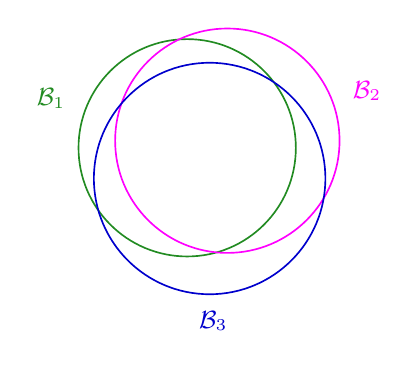
\begin{tikzpicture}[scale=1.5]
        \draw[semithick, draw=ForestGreen] (0,0) circle (0.92);
        \draw[semithick, draw=Magenta] (0.34,0.06) circle (0.95);
        \draw[semithick, draw=blue!80!black] (0.19,-0.26) circle (0.98);
        \node[font=\small, text=ForestGreen, left] at (-0.95,0.42)
            {\(\mathcal{B}_1\)};
        \node[font=\small, text=Magenta, right] at (1.32,0.48)
            {\(\mathcal{B}_2\)};
        \node[font=\small, text=blue!80!black, below] at (0.22,-1.30)
            {\(\mathcal{B}_3\)};
    \end{tikzpicture}
\end{center}

Three BAD events that nearly coincide are charged as three, and with a
continuum of lines the overcharging is unbounded --- which is precisely how a
finite quantity turned into \(\infty\).

\begin{question}\label{q:group-by-kind}
    To account for the overlap, can we group similar hypotheses by \emph{kind}?
\end{question}

\subsection{How Many Lines Are There?}

Take \(\mathcal{H} = \left\{ \text{all lines in } \mathbb{R}^2 \right\}\), where
each line is read as a hypothesis by calling one side \(\circ\) and the other
\(\times\). How many lines? Infinitely many. But the question worth asking is
not how many lines exist; it is how many of them a handful of inputs can tell
apart.

Viewed from a single input vector \(\bm{x}_1\), a line is nothing but the answer
it gives at that one point.

\begin{center}
    \begin{tikzpicture}[scale=0.95]
        \draw[dashed, black!60] (0,0) rectangle (3.2,3.0);
        \draw[black!45] (0.00,0.30) -- (3.20,1.3667);
        \draw[black!45] (0.35,0.00) -- (1.75,3.00);
        \draw[wvec, draw=blue!55] (1.80,0.90) -- ++(-0.20,0.62);
        \node[font=\small, text=black!55] at (2.34,0.76) {\(h_1\)};
        \draw[wvec, draw=blue!55] (1.12,1.65) -- ++(-0.60,0.28);
        \node[font=\small, text=black!55] at (0.74,1.48) {\(h_2\)};
        \node[circle, fill=black, inner sep=1.1pt] at (2.05,2.15) {};
        \node[right, font=\small] at (2.12,2.22) {\(\bm{x}_1\)};
    \end{tikzpicture}
    \qquad
    \(\Longrightarrow\;\; 2\colon\)\quad
    \dichone{o}\quad\dichone{x}
\end{center}

The arrow on each line is the side it calls positive. \(h_1\) puts
\(\bm{x}_1\) on its positive side and \(h_2\) does not, so through the eye of
one input there are exactly \emph{two} kinds of line:
\(h_1\text{-like}(\bm{x}_1) = \circ\) or
\(h_2\text{-like}(\bm{x}_1) = \times\). Every one of the infinitely many lines
is one or the other.

Add a second input and the eye gets sharper.

\begin{center}
    \begin{tikzpicture}[scale=0.95]
        \draw[dashed, black!60] (0,0) rectangle (3.2,3.0);
        \draw[black!45] (0.1219,0.00) -- (3.20,0.9657);
        \draw[black!45] (0.25,0.00) -- (1.55,3.00);
        \draw[sepline] (0.00,1.75) -- (3.20,1.75);
        \draw[wvec, draw=blue!55] (1.059,0.294) -- ++(-0.195,0.620);
        \node[font=\small, text=black!55] at (1.76,0.16) {\(h_1\)};
        \draw[wvec, draw=blue!55] (1.225,2.250) -- ++(-0.596,0.258);
        \node[font=\small, text=black!55] at (1.70,2.64) {\(h_2\)};
        \draw[wvec, draw=blue!75!black] (2.92,1.75) -- ++(0,0.56);
        \node[font=\small, above] at (2.92,2.33) {\(h_3\)};
        \draw[wvec, draw=blue!75!black] (2.52,1.75) -- ++(0,-0.56);
        \node[font=\small, below] at (2.52,1.24) {\(h_4\)};
        \node[circle, fill=black, inner sep=1.1pt] at (2.05,2.15) {};
        \node[above left, font=\small, inner sep=1.5pt] at (2.05,2.15) {\(\bm{x}_1\)};
        \node[circle, fill=black, inner sep=1.1pt] at (1.25,1.35) {};
        \node[below right, font=\small, inner sep=1.5pt] at (1.25,1.35) {\(\bm{x}_2\)};
    \end{tikzpicture}
    \qquad
    \(\Longrightarrow\;\; 4\colon\)\quad
    \dichtwo{oo}\;\dichtwo{xx}\;\dichtwo{ox}\;\dichtwo{xo}
\end{center}

\(h_1\) leaves both points on its positive side and \(h_2\) leaves both on its
negative side; the horizontal line between them, read upwards as \(h_3\) and
downwards as \(h_4\), splits them the two possible ways. Four kinds, one for
each of the \(2^2\) ways to label two points --- and here the count is exactly
\(2^2\), which will not last.

\begin{question}\label{q:three-inputs}
    One input: \(2\); two inputs: \(4\). Three inputs?
\end{question}

\subsection{Three Inputs, and Why the Answer Is Not One Number}

For three inputs in general position --- a genuine triangle --- every one of the
\(2^3\) labellings is achievable, because any single vertex can be cut off from
the other two by a line, and so can any pair.

\begin{center}
    \begin{tabular}{@{}c@{\quad}c@{\quad}c@{}}
        \begin{tikzpicture}[scale=0.95, baseline=(current bounding box.center)]
            \draw[dashed, black!60] (0,0) rectangle (3.2,3.0);
            \node[circle, fill=black, inner sep=1.1pt] at (1.75,2.20) {};
            \node[right, font=\small] at (1.82,2.27) {\(\bm{x}_1\)};
            \node[circle, fill=black, inner sep=1.1pt] at (0.75,1.45) {};
            \node[right, font=\small] at (0.82,1.38) {\(\bm{x}_2\)};
            \node[circle, fill=black, inner sep=1.1pt] at (2.35,0.75) {};
            \node[right, font=\small] at (2.42,0.68) {\(\bm{x}_3\)};
        \end{tikzpicture}
        & \(\Longrightarrow\; 8\colon\) &
        \begin{tabular}{@{}c@{\;}c@{\;}c@{\;}c@{}}
            \dichthree{ooo} & \dichthree{oox} & \dichthree{oxo} & \dichthree{oxx}\\
            \dichthree{xxx} & \dichthree{xxo} & \dichthree{xox} & \dichthree{xoo}
        \end{tabular}
    \end{tabular}
\end{center}

Move the three inputs onto a common line, though, and two of the eight
evaporate.

\begin{center}
    \begin{tabular}{@{}c@{\quad}c@{\quad}c@{}}
        \begin{tikzpicture}[scale=0.95, baseline=(current bounding box.center)]
            \draw[dashed, black!60] (0,0) rectangle (3.2,3.0);
            \node[circle, fill=black, inner sep=1.1pt] at (2.05,2.20) {};
            \node[right, font=\small] at (2.12,2.27) {\(\bm{x}_1\)};
            \node[circle, fill=black, inner sep=1.1pt] at (1.35,1.50) {};
            \node[right, font=\small] at (1.42,1.43) {\(\bm{x}_2\)};
            \node[circle, fill=black, inner sep=1.1pt] at (0.65,0.80) {};
            \node[right, font=\small] at (0.72,0.73) {\(\bm{x}_3\)};
        \end{tikzpicture}
        & \(\Longrightarrow\; 6\colon\) &
        \begin{tabular}{@{}c@{\;}c@{\;}c@{\;}c@{}}
            \dichcol{ooo} & \dichcol{oox} & \dichcol[veto]{oxo} & \dichcol{oxx}\\
            \dichcol{xxx} & \dichcol{xxo} & \dichcol[veto]{xox} & \dichcol{xoo}
        \end{tabular}
    \end{tabular}
\end{center}

\begin{observation}
    The two struck-out panels are the two that ask the middle point to differ
    from both of its neighbours. A line meets the segment
    \(\bm{x}_1 \bm{x}_3\) at most once, so it can never put \(\bm{x}_2\) alone
    on one side of it. `Fewer than \(8\)' is what degeneracy --- collinear
    inputs, or repeated ones --- costs.
\end{observation}

So the number of kinds depends on \emph{which} three inputs we look through, and
the two answers are \(8\) and \(6\). We will take the larger one, for a reason
that becomes clear in \autoref{sec:effective-hyp}: the bound has to hold for
every data set, so the count that goes into it must be the worst case.

\subsection{Four Inputs}

With four inputs the maximum stops keeping up with \(2^N\) for the first time.
In theory there are \(2^4 = 16\) labellings to account for, yet the picture
below draws only eight of them. Nothing is being hidden: a line read from its
other side calls every \(\circ\) a \(\times\) and every \(\times\) a \(\circ\),
so the dichotomies come in complementary pairs and one panel does for both
members of a pair. That is what the `\(2\times\)' beside the figure means, and
it is why the eight panels drawn are exactly the eight with
\(\bm{x}_1 = \circ\).

\begin{center}
    \begin{tabular}{@{}c@{\quad}c@{\quad}c@{}}
        \begin{tikzpicture}[scale=0.95, baseline=(current bounding box.center)]
            \draw[dashed, black!60] (0,0) rectangle (3.2,3.0);
            \node[circle, fill=black, inner sep=1.1pt] at (1.55,2.25) {};
            \node[above left, font=\small, inner sep=1.5pt] at (1.55,2.25)
                {\(\bm{x}_1\)};
            \node[circle, fill=black, inner sep=1.1pt] at (0.80,1.45) {};
            \node[left, font=\small, inner sep=2pt] at (0.80,1.45) {\(\bm{x}_2\)};
            \node[circle, fill=black, inner sep=1.1pt] at (1.95,0.70) {};
            \node[below, font=\small, inner sep=2pt] at (1.95,0.70) {\(\bm{x}_3\)};
            \node[circle, fill=black, inner sep=1.1pt] at (2.45,1.60) {};
            \node[right, font=\small, inner sep=2pt] at (2.45,1.60) {\(\bm{x}_4\)};
        \end{tikzpicture}
        & \(\Longrightarrow\; 14 \colon 2 \times\) &
        \begin{tabular}{@{}c@{\;}c@{\;}c@{\;}c@{}}
            \dichfour{oooo} & \dichfour{ooox} & \dichfour{ooxo}
            & \dichfour[veto]{oxox}\\
            \dichfour{ooxx} & \dichfour{oxxo} & \dichfour{oxoo}
            & \dichfour{oxxx}
        \end{tabular}
    \end{tabular}
\end{center}

Of the sixteen, exactly one pair is missing: the struck-out panel, which asks
\(\bm{x}_1\) and \(\bm{x}_3\) to differ from \(\bm{x}_2\) and \(\bm{x}_4\),
together with its mirror image. Fourteen survive.

\begin{proposition}[At most \(14\) through four inputs]\label{prop:fourteen}
    For any four inputs \(\bm{x}_1, \dots , \bm{x}_4 \in \mathbb{R}^2\), lines
    realise at most \(14\) of the \(2^4 = 16\) labellings, and \(14\) is
    attained.
\end{proposition}

\begin{proof}
    Radon's theorem says that any four points of \(\mathbb{R}^2\) can be
    partitioned into two groups whose convex hulls intersect. Fix such a
    partition and colour one group \(\circ\) and the other \(\times\). A line
    realising that labelling would separate the two groups, hence separate their
    convex hulls --- impossible, since the hulls share a point. The same
    partition with the colours exchanged is a second labelling ruled out for the
    same reason, and it is a different labelling because a group and its
    complement are never equal. So at least two of the \(16\) are missing.

    The picture above attains the bound: the four points are in convex position
    in the cyclic order \(\bm{x}_1, \bm{x}_4, \bm{x}_3, \bm{x}_2\), the
    intersecting hulls are the two diagonals \(\bm{x}_1 \bm{x}_3\) and
    \(\bm{x}_2 \bm{x}_4\), and every other labelling is cut off by a line.
\end{proof}

\begin{remark}
    The degenerate configurations do no better. If one input lies inside the
    triangle of the other three, Radon's partition is `inner point against the
    rest' and again removes exactly two labellings; if three of them are
    collinear, more labellings are lost, not fewer. Four inputs never see more
    than \(14\) kinds of line, which is the first crack in the ceiling
    \(2^N\).
\end{remark}

\subsection{Effective Number of Lines}

\begin{definition}[Effective number of lines]\label{def:effective}
    The \vocab{effective number of lines} for \(N\) inputs is the maximum number
    of kinds of lines with respect to any \(N\) inputs
    \(\bm{x}_1, \bm{x}_2, \dots , \bm{x}_N\), written
    \(\operatorname{effective}(N)\).
\end{definition}

Three facts come for free. It must be at most \(2^N\), since a kind of line is
no more than an assignment of one of two labels to each of \(N\) inputs. It is a
finite grouping of the infinitely many lines in \(\mathcal{H}\), which is
exactly what \autoref{q:group-by-kind} asked for. And the counts collected so
far are

\begin{center}
    \solidrules
    \begin{tabular}{@{}c|c@{}}
        \toprule
        \multicolumn{2}{@{}c@{}}{\textbf{lines in 2D}}\\
        \midrule
        \(N\) & \(\operatorname{effective}(N)\)\\
        \midrule
        \(1\) & \(2\)\\
        \(2\) & \(4\)\\
        \(3\) & \(8\)\\
        \(4\) & \(14 < 2^N\)\\
        \bottomrule
    \end{tabular}
\end{center}

The wish is then easy to state: that the proof of
\autoref{thm:finite-hoeffding} could be rerun with the number of kinds in place
of the number of hypotheses, giving
\[
    \mathbb{P}\left[ \abs{\Ein(g) - \Eout(g)} > \epsilon \right]
    \le 2 \cdot \operatorname{effective}(N) \cdot \exp \left( -2 \epsilon^2 N \right) .
\]

\begin{moral}
    If \raisebox{0pt}[0pt][0pt]{\textcircled{\scriptsize 1}}
    \(\operatorname{effective}(N)\) can replace \(M\) and
    \raisebox{0pt}[0pt][0pt]{\textcircled{\scriptsize 2}}
    \(\operatorname{effective}(N) \ll 2^N\), then learning is possible with
    infinitely many lines. :-)
\end{moral}

\begin{intuition}
    Why both conditions? The first is the replacement itself. The second is what
    makes the replacement worth having: \(\exp(-2\epsilon^2 N)\) decays
    exponentially in \(N\), so a factor growing like \(2^N\) would cancel it
    exactly and leave a bound that never becomes small. Anything that grows
    polynomially loses the race and the product still vanishes.
\end{intuition}

\begin{exercise}[Fun Time]
    What is the effective number of lines for five inputs in \(\mathbb{R}^2\)?
    \begin{enumerate*}[(1)]
        \item \(14\); \item \(16\); \item \(22\); \item \(32\).
    \end{enumerate*}
\end{exercise}

\begin{proof}[Reference Answer]
    (3). If you put the inputs roughly around a circle,

    \begin{center}
        \begin{tikzpicture}[scale=0.95]
            \draw[dashed, black!60] (0,0) rectangle (3.2,3.0);
            \node[circle, fill=black, inner sep=1.1pt] at (1.285,2.436) {};
            \node[above, font=\small] at (1.26,2.50) {\(\bm{x}_1\)};
            \node[circle, fill=black, inner sep=1.1pt] at (0.514,1.665) {};
            \node[left, font=\small] at (0.45,1.66) {\(\bm{x}_2\)};
            \node[circle, fill=black, inner sep=1.1pt] at (1.851,0.639) {};
            \node[right, font=\small] at (1.92,0.62) {\(\bm{x}_3\)};
            \node[circle, fill=black, inner sep=1.1pt] at (2.396,1.583) {};
            \node[right, font=\small] at (2.46,1.57) {\(\bm{x}_4\)};
            \node[circle, fill=black, inner sep=1.1pt] at (2.228,2.045) {};
            \node[right, font=\small] at (2.29,2.06) {\(\bm{x}_5\)};
        \end{tikzpicture}
    \end{center}

    you can then pick any \emph{consecutive} run of inputs to be on one side of
    the line, and the rest on the other. There are \(5 \cdot 4 = 20\) proper
    runs --- five starting points times four lengths --- plus the two labellings
    that use no line at all, all \(\circ\) and all \(\times\), for a total of
    \(22\) kinds, much smaller than \(2^5 = 32\). You will find it difficult to
    generate more kinds by varying the inputs, and a formal proof comes in a
    later chapter.
\end{proof}

\begin{remark}
    The counts \(2, 4, 8, 14, 22\) are the start of
    \(2 \left[ \binom{N-1}{0} + \binom{N-1}{1} + \binom{N-1}{2} \right]\), which
    is Cover's formula for the number of dichotomies of \(N\) points in general
    position realisable by a hyperplane in the plane. The differences
    \(2, 4, 6, 8\) between consecutive terms are the giveaway: a quadratic, not
    an exponential.
\end{remark}

\section{Effective Number of Hypotheses}\label{sec:effective-hyp}

\source{slides p.16--22}

Everything in the previous section was about lines. Nothing in it was, and the
same counting works for any hypothesis set at all once the vocabulary is
detached from geometry.

\subsection{Dichotomies: Mini-hypotheses}

Let \(\mathcal{H}\) be any set of hypotheses \(h \colon \mathcal{X} \to
\left\{ \times, \circ \right\}\).

\begin{definition}[Dichotomy]\label{def:dichotomy}
    For fixed inputs \(\bm{x}_1, \dots , \bm{x}_N\), write
    \[
        h(\bm{x}_1, \bm{x}_2, \dots , \bm{x}_N)
        = \left( h(\bm{x}_1), h(\bm{x}_2), \dots , h(\bm{x}_N) \right)
        \in \left\{ \times, \circ \right\}^N ,
    \]
    and call it a \vocab{dichotomy}: the hypothesis `limited' to the eyes of the
    \(N\) inputs. Write
    \[
        \mathcal{H}(\bm{x}_1, \bm{x}_2, \dots , \bm{x}_N)
    \]
    for the set of all dichotomies implemented by \(\mathcal{H}\) on them.
\end{definition}

\begin{notation}
    A dichotomy is written as a string, one symbol per input in index order:
    \(\circ\circ\times\circ\) is the dichotomy that answers \(\circ\) on
    \(\bm{x}_1, \bm{x}_2, \bm{x}_4\) and \(\times\) on \(\bm{x}_3\). The panels
    of \autoref{sec:effective-lines} are exactly such strings, drawn.
\end{notation}

A dichotomy is a mini-hypothesis: all of \(h\) that \(N\) inputs can possibly
detect. Two hypotheses collapse into one dichotomy precisely when the inputs
cannot tell them apart --- which is the overlap of \autoref{q:union-fail}, now
made into an object. That sentence is the whole reason for the definition, so
it is worth making exact.

\begin{lemma}[Same dichotomy, same \texorpdfstring{\(\Ein\)}{Ein}]\label{lem:same-ein}
    If \(h\) and \(h'\) implement the same dichotomy on the inputs of
    \(\mathcal{D}\), then \(\Ein(h) = \Ein(h')\) --- not approximately, exactly.
\end{lemma}

\begin{proof}
    \(\Ein(h) = \frac{1}{N} \sum_{n=1}^{N}
    \llbracket h(\bm{x}_n) \neq y_n \rrbracket\) by \autoref{def:errors},
    and by hypothesis \(h(\bm{x}_n) = h'(\bm{x}_n)\) for every \(n\), so the two
    sums have the same terms.
\end{proof}

Now retrace where \(M\) came from. It was a count of summands in the union
bound of \autoref{sec:effective-lines}, one for each BAD event
\(\mathcal{B}_h \colon \abs{\Ein(h) - \Eout(h)} > \epsilon\). The hypotheses
sharing a dichotomy have the same \(\Ein\) by \autoref{lem:same-ein}, and ---
agreeing wherever the data looks --- nearly the same \(\Eout\); their BAD events
therefore nearly coincide, exactly the three-circle picture of
\autoref{sec:effective-lines}. Such a family deserves one summand between all of
its members, not one each. Charge per \emph{dichotomy} instead of per hypothesis
and the number of summands falls from \(\abs{\mathcal{H}}\) to
\(\abs{\mathcal{H}(\bm{x}_1, \bm{x}_2, \dots , \bm{x}_N)}\), which is at most
\(2^N\) however infinite \(\mathcal{H}\) may be.

\begin{center}
    \solidrules
    \begin{adjustbox}{max width=\textwidth}
        \begin{tabular}{@{}c|c|c@{}}
            \toprule
            & hypotheses \(\mathcal{H}\)
            & dichotomies \(\mathcal{H}(\bm{x}_1, \bm{x}_2, \dots , \bm{x}_N)\)\\
            \midrule
            e.g.\ & all lines in \(\mathbb{R}^2\)
            & \(\left\{ \circ\circ\circ\circ , \circ\circ\circ\times ,
                \circ\circ\times\times , \dots \right\}\)\\
            size & possibly infinite & upper bounded by \(2^N\)\\
            \bottomrule
        \end{tabular}
    \end{adjustbox}
\end{center}

\begin{moral}
    \(\abs{\mathcal{H}(\bm{x}_1, \bm{x}_2, \dots , \bm{x}_N)}\) is our candidate
    for replacing \(M\).
\end{moral}

\begin{note}
    `Candidate' is the honest word, because the grouping argument above is a
    motivation and not yet a proof. Two things are missing. The set
    \(\mathcal{H}(\bm{x}_1, \bm{x}_2, \dots , \bm{x}_N)\) depends on the very
    inputs we are averaging over, so it is not a fixed number a bound may quote;
    the next subsection removes that dependence. And a dichotomy pins \(\Ein\)
    exactly while leaving \(\Eout\) only \emph{approximately} equal across the
    group, so the members of a group do not literally share one BAD event and
    the union bound over groups is not yet licensed. That second gap is what the
    `\(?\)' of \autoref{eq:wish} stands for, and closing it takes until two
    chapters from now.
\end{note}

\subsection{Growth Function}

The candidate has one defect, and \autoref{sec:effective-lines} already showed
it: \(\abs{\mathcal{H}(\bm{x}_1, \dots , \bm{x}_N)}\) depends on which inputs
are chosen --- \(8\) for a triangle, \(6\) for three collinear points. A bound
cannot depend on a data set it is supposed to hold for, so the dependence is
removed in the only safe direction.

\begin{definition}[Growth function]\label{def:growth}
    The \vocab{growth function} of \(\mathcal{H}\) is
    \[
        m_{\mathcal{H}}(N)
        = \max_{\bm{x}_1, \bm{x}_2, \dots , \bm{x}_N \in \mathcal{X}}
        \abs{\mathcal{H}(\bm{x}_1, \bm{x}_2, \dots , \bm{x}_N)} .
    \]
\end{definition}

It is finite and upper bounded by \(2^N\), so unlike \(M\) it never escapes to
infinity, however large \(\mathcal{H}\) is. For lines in the plane it is the
effective number of \autoref{def:effective}:

\begin{center}
    \solidrules
    \begin{tabular}{@{}c|c@{}}
        \toprule
        \multicolumn{2}{@{}c@{}}{\textbf{lines in 2D}}\\
        \midrule
        \(N\) & \(m_{\mathcal{H}}(N)\)\\
        \midrule
        \(1\) & \(2\)\\
        \(2\) & \(4\)\\
        \(3\) & \(\max(\dots , 6, 8) = 8\)\\
        \(4\) & \(14 < 2^N\)\\
        \bottomrule
    \end{tabular}
\end{center}

The \(\max\) in the third row is the definition doing its job: the degenerate
configurations are still there, they are simply not the ones that decide.

\begin{question}\label{q:calculate-growth}
    How does one actually `calculate' the growth function?
\end{question}

The honest answer is that for perceptrons we cannot yet, so the next three
subsections take hypothesis sets simple enough to count by hand. Each is chosen
to land somewhere different on the scale from polynomial to exponential.

\subsection{Growth Function for Positive Rays}

Let \(\mathcal{X} = \mathbb{R}\) be one dimensional and let \(\mathcal{H}\)
contain every \(h(x) = \sign(x - a)\) for a threshold \(a \in \mathbb{R}\) ---
the `positive half' of the 1D perceptrons.

\begin{center}
    \begin{tikzpicture}[scale=1.0]
        \draw[black!70] (-0.10,0) -- (8.60,0);
        \foreach \x in {0.7,1.5,2.3,3.9}{\node[dneg] at (\x,0) {\(\times\)};}
        \foreach \x in {4.9,5.7,6.5,7.6}{\node[dpos] at (\x,0) {};}
        \node[font=\small] at (3.1,0) {\(\dots\)};
        \node[below, font=\scriptsize] at (0.7,-0.14) {\(x_1\)};
        \node[below, font=\scriptsize] at (1.5,-0.14) {\(x_2\)};
        \node[below, font=\scriptsize] at (2.3,-0.14) {\(x_3\)};
        \node[below, font=\scriptsize] at (7.6,-0.14) {\(x_N\)};
        \draw[dashed, black!55] (4.4,-0.30) -- (4.4,1.00);
        \node[font=\small, text=black!70] at (4.24,1.16) {\(a\)};
        \draw[-{Stealth[length=2.0mm]}, semithick, draw=blue!70!black]
            (4.42,1.00) -- (8.50,1.00);
        \node[font=\small, text=red!85!black] at (2.2,0.58)
            {\(h(x) = -1\)};
        \node[font=\small, text=blue!70!black] at (6.4,0.58)
            {\(h(x) = +1\)};
    \end{tikzpicture}
\end{center}

\begin{proposition}[Positive rays]\label{prop:rays}
    \(m_{\mathcal{H}}(N) = N + 1\).
\end{proposition}

\begin{proof}
    Sort the inputs as \(x_1 < x_2 < \dots < x_N\). The dichotomy produced by
    threshold \(a\) depends only on how many inputs lie below \(a\), so all
    thresholds inside one gap \((x_n, x_{n+1})\) give the same dichotomy, and
    different gaps give different ones. There are \(N + 1\) gaps --- the \(N-1\)
    internal ones together with \((-\infty, x_1)\) and \((x_N, \infty)\) ---
    hence \(N + 1\) dichotomies, and no choice of inputs does better, since
    repeated inputs only merge gaps.
\end{proof}

For \(N = 4\) the \(5\) dichotomies are all the ways to put the crosses first:

\begin{center}
    \begin{tabular}{@{}cccc@{}}
        \toprule
        \(x_1\) & \(x_2\) & \(x_3\) & \(x_4\)\\
        \midrule
        \dmark{o} & \dmark{o} & \dmark{o} & \dmark{o}\\
        \dmark{x} & \dmark{o} & \dmark{o} & \dmark{o}\\
        \dmark{x} & \dmark{x} & \dmark{o} & \dmark{o}\\
        \dmark{x} & \dmark{x} & \dmark{x} & \dmark{o}\\
        \dmark{x} & \dmark{x} & \dmark{x} & \dmark{x}\\
        \bottomrule
    \end{tabular}
\end{center}

\begin{moral}
    \((N + 1) \ll 2^N\) when \(N\) is large.
\end{moral}

\subsection{Growth Function for Positive Intervals}

Keep \(\mathcal{X} = \mathbb{R}\) and let \(\mathcal{H}\) contain every \(h\)
with \(h(x) = +1\) if and only if \(x \in [\ell, r)\), and \(-1\) otherwise.

\begin{center}
    \begin{tikzpicture}[scale=1.0]
        \draw[black!70] (-0.10,0) -- (9.30,0);
        \foreach \x in {0.7,1.5,2.3,3.9}{\node[dneg] at (\x,0) {\(\times\)};}
        \foreach \x in {4.9,5.6,6.3}{\node[dpos] at (\x,0) {};}
        \node[dneg] at (8.4,0) {\(\times\)};
        \node[font=\small] at (3.1,0) {\(\dots\)};
        \node[below, font=\scriptsize] at (0.7,-0.14) {\(x_1\)};
        \node[below, font=\scriptsize] at (1.5,-0.14) {\(x_2\)};
        \node[below, font=\scriptsize] at (2.3,-0.14) {\(x_3\)};
        \node[below, font=\scriptsize] at (8.4,-0.14) {\(x_N\)};
        \draw[dashed, black!55] (4.45,-0.28) -- (4.45,1.06);
        \draw[dashed, black!55] (6.90,-0.28) -- (6.90,1.06);
        \node[font=\small, text=black!70] at (4.29,1.22) {\(\ell\)};
        \node[font=\small, text=black!70] at (7.06,1.22) {\(r\)};
        \draw[{Stealth[length=2.0mm]}-{Stealth[length=2.0mm]}, semithick,
            draw=blue!70!black] (4.47,1.06) -- (6.88,1.06);
        \node[font=\small, text=red!85!black] at (2.2,0.58) {\(h(x) = -1\)};
        \node[font=\small, text=blue!70!black] at (5.67,0.58) {\(h(x) = +1\)};
        \node[font=\small, text=red!85!black] at (8.55,0.58) {\(h(x) = -1\)};
    \end{tikzpicture}
\end{center}

\begin{proposition}[Positive intervals]\label{prop:intervals}
    \(m_{\mathcal{H}}(N) = \binom{N+1}{2} + 1 = \tfrac{1}{2} N^2 +
    \tfrac{1}{2} N + 1\).
\end{proposition}

\begin{proof}
    As before, only the gaps matter: a dichotomy is decided by which of the
    \(N + 1\) spots holds \(\ell\) and which holds \(r\). Choosing two
    \emph{different} spots for the two ends, with \(\ell\) in the earlier one,
    gives \(\binom{N+1}{2}\) distinct dichotomies, each with a non-empty run of
    \(\circ\). Putting both ends in the same spot makes the interval miss every
    input and produces the all-\(\times\) dichotomy, one further case however the
    spot is chosen. Adding the two counts gives
    \(\binom{N+1}{2} + 1\).
\end{proof}

For \(N = 4\) that is \(10 + 1 = 11\): every contiguous run of \(\circ\), plus
the empty one.

\begin{center}
    \begin{tabular}[t]{@{}cccc@{}}
        \toprule
        \(x_1\) & \(x_2\) & \(x_3\) & \(x_4\)\\
        \midrule
        \dmark{o} & \dmark{x} & \dmark{x} & \dmark{x}\\
        \dmark{o} & \dmark{o} & \dmark{x} & \dmark{x}\\
        \dmark{o} & \dmark{o} & \dmark{o} & \dmark{x}\\
        \dmark{o} & \dmark{o} & \dmark{o} & \dmark{o}\\
        \dmark{x} & \dmark{o} & \dmark{x} & \dmark{x}\\
        \dmark{x} & \dmark{o} & \dmark{o} & \dmark{x}\\
        \bottomrule
    \end{tabular}
    \qquad\qquad
    \begin{tabular}[t]{@{}cccc@{}}
        \toprule
        \(x_1\) & \(x_2\) & \(x_3\) & \(x_4\)\\
        \midrule
        \dmark{x} & \dmark{o} & \dmark{o} & \dmark{o}\\
        \dmark{x} & \dmark{x} & \dmark{o} & \dmark{x}\\
        \dmark{x} & \dmark{x} & \dmark{o} & \dmark{o}\\
        \dmark{x} & \dmark{x} & \dmark{x} & \dmark{o}\\
        \dmark{x} & \dmark{x} & \dmark{x} & \dmark{x}\\
        \bottomrule
    \end{tabular}
\end{center}

\begin{moral}
    \(\left( \tfrac{1}{2} N^2 + \tfrac{1}{2} N + 1 \right) \ll 2^N\) when \(N\)
    is large.
\end{moral}

\subsection{Growth Function for Convex Sets}

Now let \(\mathcal{X} = \mathbb{R}^2\) and let \(\mathcal{H}\) contain every
\(h\) with \(h(\bm{x}) = +1\) if and only if \(\bm{x}\) lies in a convex region,
and \(-1\) otherwise. Blue marks the region a hypothesis calls \(+1\); the red
surround is everything it calls \(-1\).

\begin{center}
    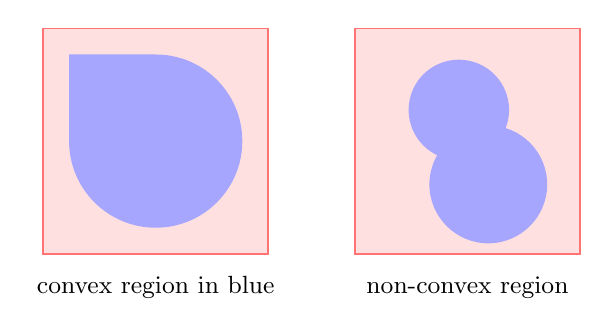
\begin{tikzpicture}[scale=1.1]
        \fill[red!12, draw=red!55, semithick] (-1.3,-1.3) rectangle (1.3,1.3);
        \fill[blue!35] (-1,0) -- (-1,1) -- (0,1)
            arc[start angle=90, end angle=-180, radius=1] -- cycle;
        \node[below, font=\small] at (0,-1.45) {convex region in blue};
        \begin{scope}[xshift=3.6cm]
            \fill[red!12, draw=red!55, semithick] (-1.3,-1.3) rectangle (1.3,1.3);
            \fill[blue!35] (-0.10,0.36) circle (0.58);
            \fill[blue!35] (0.24,-0.50) circle (0.68);
            \node[below, font=\small] at (0,-1.45) {non-convex region};
        \end{scope}
    \end{tikzpicture}
\end{center}

\begin{question}\label{q:convex-growth}
    What is \(m_{\mathcal{H}}(N)\) for convex sets?
\end{question}

The answer is the ceiling, and the way to see it is to choose the inputs as
favourably as the \(\max\) in \autoref{def:growth} permits: put
\(\bm{x}_1, \bm{x}_2, \dots , \bm{x}_N\) on a big circle.

\begin{center}
    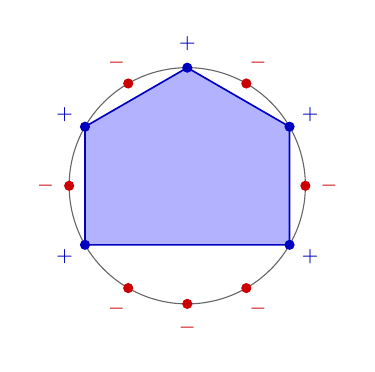
\begin{tikzpicture}[scale=1.5]
        \draw[black!60] (0,0) circle (1);
        \fill[blue!30, draw=blue!75!black, semithick]
            (30:1) -- (90:1) -- (150:1) -- (210:1) -- (330:1) -- cycle;
        \foreach \a in {30,90,150,210,330}{
            \node[circle, fill=blue!75!black, inner sep=1.3pt] at (\a:1) {};
            \node[font=\scriptsize, text=blue!75!black] at (\a:1.20) {\(+\)};}
        \foreach \a in {0,60,120,180,240,270,300}{
            \node[circle, fill=red!80!black, inner sep=1.3pt] at (\a:1) {};
            \node[font=\scriptsize, text=red!80!black] at (\a:1.20) {\(-\)};}
    \end{tikzpicture}
\end{center}

\begin{proposition}[Convex sets]\label{prop:convex}
    \(m_{\mathcal{H}}(N) = 2^N\).
\end{proposition}

\begin{proof}
    Place the \(N\) inputs on a circle and fix any dichotomy. Take the convex
    hull of the inputs labelled \(+1\) and extend it very slightly. Every
    positive input is inside by construction. Every negative input is outside,
    because a point of a circle is a vertex of the convex hull of any subset of
    that circle containing it --- so it cannot lie in the hull of a subset that
    excludes it. The region is convex, so it is a legitimate \(h\), and it
    implements the chosen dichotomy. All \(2^N\) dichotomies are therefore
    implemented by these inputs, and \(2^N\) is also the ceiling.
\end{proof}

\begin{definition}[Shattering]\label{def:shatter}
    When \(\mathcal{H}\) implements every one of the \(2^N\) dichotomies on
    \(\bm{x}_1, \dots , \bm{x}_N\), those \(N\) inputs are \vocab{shattered} by
    \(\mathcal{H}\).
\end{definition}

\begin{moral}
    \(m_{\mathcal{H}}(N) = 2^N\) if and only if there exist \(N\) inputs that
    can be shattered.
\end{moral}

\begin{remark}
    The `if and only if' is worth reading twice, because it is where the
    \(\max\) pays off. \emph{Some} choice of \(N\) inputs being shattered is
    enough; the other choices may be as degenerate as they like. Conversely, a
    growth function short of \(2^N\) is a statement about \emph{every}
    conceivable set of \(N\) inputs at once.
\end{remark}

\begin{exercise}[Fun Time]
    Consider positive \emph{and} negative rays as \(\mathcal{H}\), which is
    equivalent to the perceptron hypothesis set in 1D. The hypothesis set is
    often called a `decision stump', to describe the shape of its hypotheses.
    What is the growth function \(m_{\mathcal{H}}(N)\)?
    \begin{enumerate*}[(1)]
        \item \(N\); \item \(N + 1\); \item \(2N\); \item \(2^N\).
    \end{enumerate*}
\end{exercise}

\begin{proof}[Reference Answer]
    (3). Two dichotomies when the threshold falls in each of the \(N - 1\)
    `internal' spots, one for each reading of the sign, giving \(2(N-1)\); then
    two more for the all-\(\circ\) and all-\(\times\) cases, which the two
    outside spots produce whichever way they are read. In total
    \(2(N-1) + 2 = 2N\).
\end{proof}

\section{Break Point}\label{sec:break-point}

\source{slides p.23--26}

\subsection{The Four Growth Functions}

Four hypothesis sets, four growth functions:

\begin{itemize}
    \item positive rays: \(m_{\mathcal{H}}(N) = N + 1\);
    \item positive intervals: \(m_{\mathcal{H}}(N) = \tfrac{1}{2} N^2 +
        \tfrac{1}{2} N + 1\);
    \item convex sets: \(m_{\mathcal{H}}(N) = 2^N\);
    \item 2D perceptrons: \(m_{\mathcal{H}}(N) < 2^N\) in some cases.
\end{itemize}

Suppose \autoref{eq:wish} were granted and \(m_{\mathcal{H}}(N)\) took the
place of \(M\):
\[
    \mathbb{P}\left[ \abs{\Ein(g) - \Eout(g)} > \epsilon \right]
    \overset{?}{\le} 2 \cdot m_{\mathcal{H}}(N) \cdot
    \exp \left( -2 \epsilon^2 N \right) .
\]
The first two hypothesis sets would be safe and the third would not, and the
line between them is the only thing that matters.

\begin{moral}
    Polynomial: good; exponential: bad.
\end{moral}

\begin{question}\label{q:perceptron-poly}
    For 2D, or general, perceptrons --- is \(m_{\mathcal{H}}(N)\) polynomial?
\end{question}

\subsection{Break Point of \texorpdfstring{\(\mathcal{H}\)}{H}}

What we know about 2D perceptrons so far is two statements of opposite
quantifier. For three inputs there \emph{exists} a shattering; for four inputs,
\emph{for all} configurations, there is none.

\begin{center}
    \dichfour[veto]{oxox}
\end{center}

That second statement is the useful one, and it deserves a name.

\begin{definition}[Break point]\label{def:break}
    If no \(k\) inputs can be shattered by \(\mathcal{H}\), then \(k\) is a
    \vocab{break point} for \(\mathcal{H}\).
\end{definition}

Three consequences follow at once.

\begin{itemize}
    \item \(m_{\mathcal{H}}(k) < 2^k\), by \autoref{def:shatter}.
    \item \(k + 1, k + 2, k + 3, \dots\) are break points too.
    \item So the informative quantity is the \emph{minimum} break point, and it
        is the one we shall study.
\end{itemize}

\begin{proof}[Proof of the second bullet]
    Suppose some \(k + 1\) inputs were shattered. Delete one of them and restrict
    every dichotomy to the remaining \(k\): each of the \(2^k\) dichotomies on
    those \(k\) inputs is the restriction of at least one of the \(2^{k+1}\)
    dichotomies above it, so the \(k\) inputs are shattered as well,
    contradicting the assumption that \(k\) is a break point. Induction gives
    every larger \(k\).
\end{proof}

\begin{moral}
    2D perceptrons have a break point at \(4\).
\end{moral}

\subsection{The Four Break Points}

The same four hypothesis sets, now read for their break points:

\begin{center}
    \solidrules
    \begin{adjustbox}{max width=\textwidth}
        \begin{tabular}{@{}l|c|c@{}}
            \toprule
            \(\mathcal{H}\) & \(m_{\mathcal{H}}(N)\) & minimum break point\\
            \midrule
            positive rays & \(N + 1 = O(N)\) & \(2\)\\
            positive intervals
            & \(\tfrac{1}{2} N^2 + \tfrac{1}{2} N + 1 = O(N^2)\) & \(3\)\\
            convex sets & \(2^N\) & none\\
            2D perceptrons & \(< 2^N\) in some cases & \(4\)\\
            \bottomrule
        \end{tabular}
    \end{adjustbox}
\end{center}

The arithmetic behind the third column is a single substitution each time.
Positive rays give \(m_{\mathcal{H}}(1) = 2 = 2^1\) but
\(m_{\mathcal{H}}(2) = 3 < 4\). Positive intervals give
\(m_{\mathcal{H}}(2) = 4 = 2^2\) and \(m_{\mathcal{H}}(3) = 7 < 8\). Convex sets
never fall short of \(2^N\), so they have no break point at all. Perceptrons in
the plane shatter some three inputs and no four, by
\autoref{prop:fourteen}.

Read down the first two columns together and a pattern is hard to miss: break
point \(2\) with a linear growth function, break point \(3\) with a quadratic
one, no break point with an exponential one.

\begin{conjecture}\label{conj:break}
    No break point: \(m_{\mathcal{H}}(N) = 2^N\) --- which is certain, being the
    contrapositive of \autoref{def:break}. Break point \(k\):
    \(m_{\mathcal{H}}(N) = O \! \left( N^{k-1} \right)\).
\end{conjecture}

If the second half is true, then a single failure to shatter --- one
configuration size at which \(\mathcal{H}\) runs out of expressive power ---
forces polynomial growth for every \(N\), and with it a bound that decays.
A very small local restriction would buy a very large global guarantee. Whether
it is true is the whole of the next chapter.

\begin{exercise}[Fun Time]
    Consider positive and negative rays as \(\mathcal{H}\), the 1D perceptron
    set, whose growth function is \(m_{\mathcal{H}}(N) = 2N\). What is the
    minimum break point for \(\mathcal{H}\)?
    \begin{enumerate*}[(1)]
        \item \(1\); \item \(2\); \item \(3\); \item \(4\).
    \end{enumerate*}
\end{exercise}

\begin{proof}[Reference Answer]
    (3). At \(k = 3\) we get \(m_{\mathcal{H}}(k) = 6\) while \(2^k = 8\), so
    \(3\) is a break point; and it is minimal because \(m_{\mathcal{H}}(2) = 4 =
    2^2\) and \(m_{\mathcal{H}}(1) = 2 = 2^1\) leave nothing broken below it.
    Note that \autoref{conj:break} predicts \(O(N^2)\) here while the truth is
    \(2N\) --- the conjecture is an upper bound, not an estimate.
\end{proof}

\hrulebar

\subsection*{Summary}

\begin{description}
    \item[Recap and Preview] Two questions: \(\Eout(g) \approx \Ein(g)\), and
        \(\Ein(g) \approx 0\).
    \item[Effective Number of Lines] At most \(14\) through the eye of \(4\)
        inputs.
    \item[Effective Number of Hypotheses] At most \(m_{\mathcal{H}}(N)\) through
        the eye of \(N\) inputs.
    \item[Break Point] When \(m_{\mathcal{H}}(N)\) becomes `non-exponential'.
\end{description}

The chapter's title names the split it opened with: training is where \(\Ein\)
is made small, testing is where \(\Eout\) is judged, and the bridge between them
carries a factor that used to be \(M\). That factor is now
\(m_{\mathcal{H}}(N)\), which counts kinds of behaviour rather than hypotheses
and stays finite for the infinite hypothesis sets we care about.

Two debts remain, and they are the next two chapters. The first is
\autoref{conj:break}: a break point at \(k\) ought to force
\(m_{\mathcal{H}}(N) = O(N^{k-1})\), and until that is proved, `finite' is not
yet `polynomial'. The second is the question mark of \autoref{eq:wish}, still
sitting over
\[
    \mathbb{P}\left[ \abs{\Ein(g) - \Eout(g)} > \epsilon \right]
    \overset{?}{\le} 2 \cdot m_{\mathcal{H}}(N) \cdot
    \exp \left( -2 \epsilon^2 N \right) ,
\]
which no argument here has earned. Settle both and the perceptron --- infinite
hypothesis set and all --- finally comes with a guarantee.
